\newpage

\section{Model training / model convergence}

Consider adding implementation / log scaling here.
 
\subsection{Hyper parameters}
 
N-states, Jump penalty, times series parameters (jump model only), rolling window length
 
\subsubsection{Choosing the jump penalizer}
\label{subsection: jump_penalizer}

\begin{figure}[H] 
    \centering
    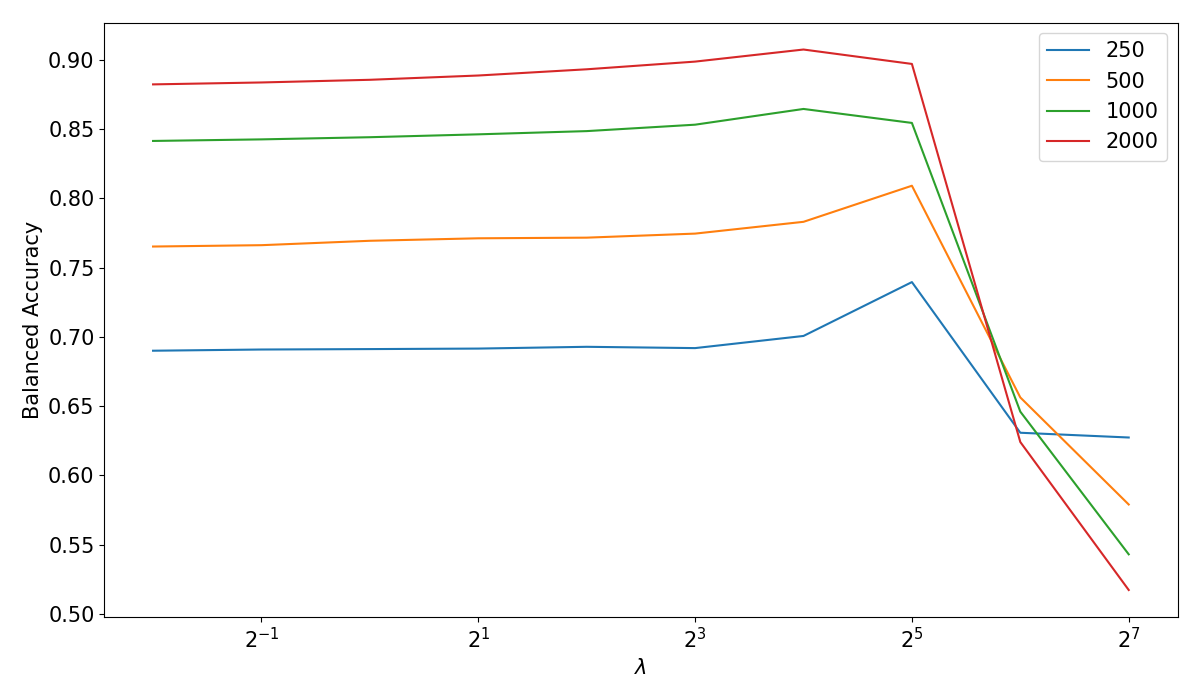
\includegraphics[width=1\textwidth]{analysis/model_convergence/images/jump_penalties.png}
    \caption{Hyper-tuning.}
    \label{fig:jump_penalties}
\end{figure}

\begin{figure}[H] 
    \centering
    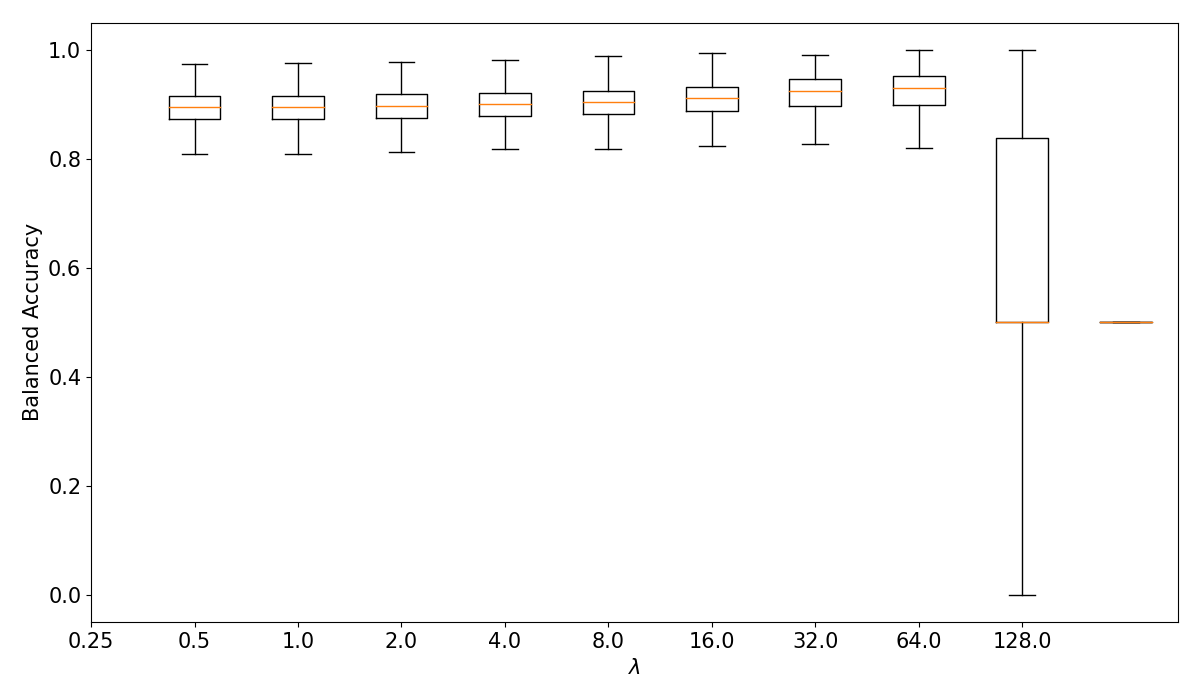
\includegraphics[width=1\textwidth]{analysis/model_convergence/images/jump_penalties_box.png}
    \caption{Hyper-tuning.}
    %\label{fig:jump_penalties}
\end{figure}


\subsection{Simulation study with correctly specified distributions}

\begin{figure}[H] 
    \centering
    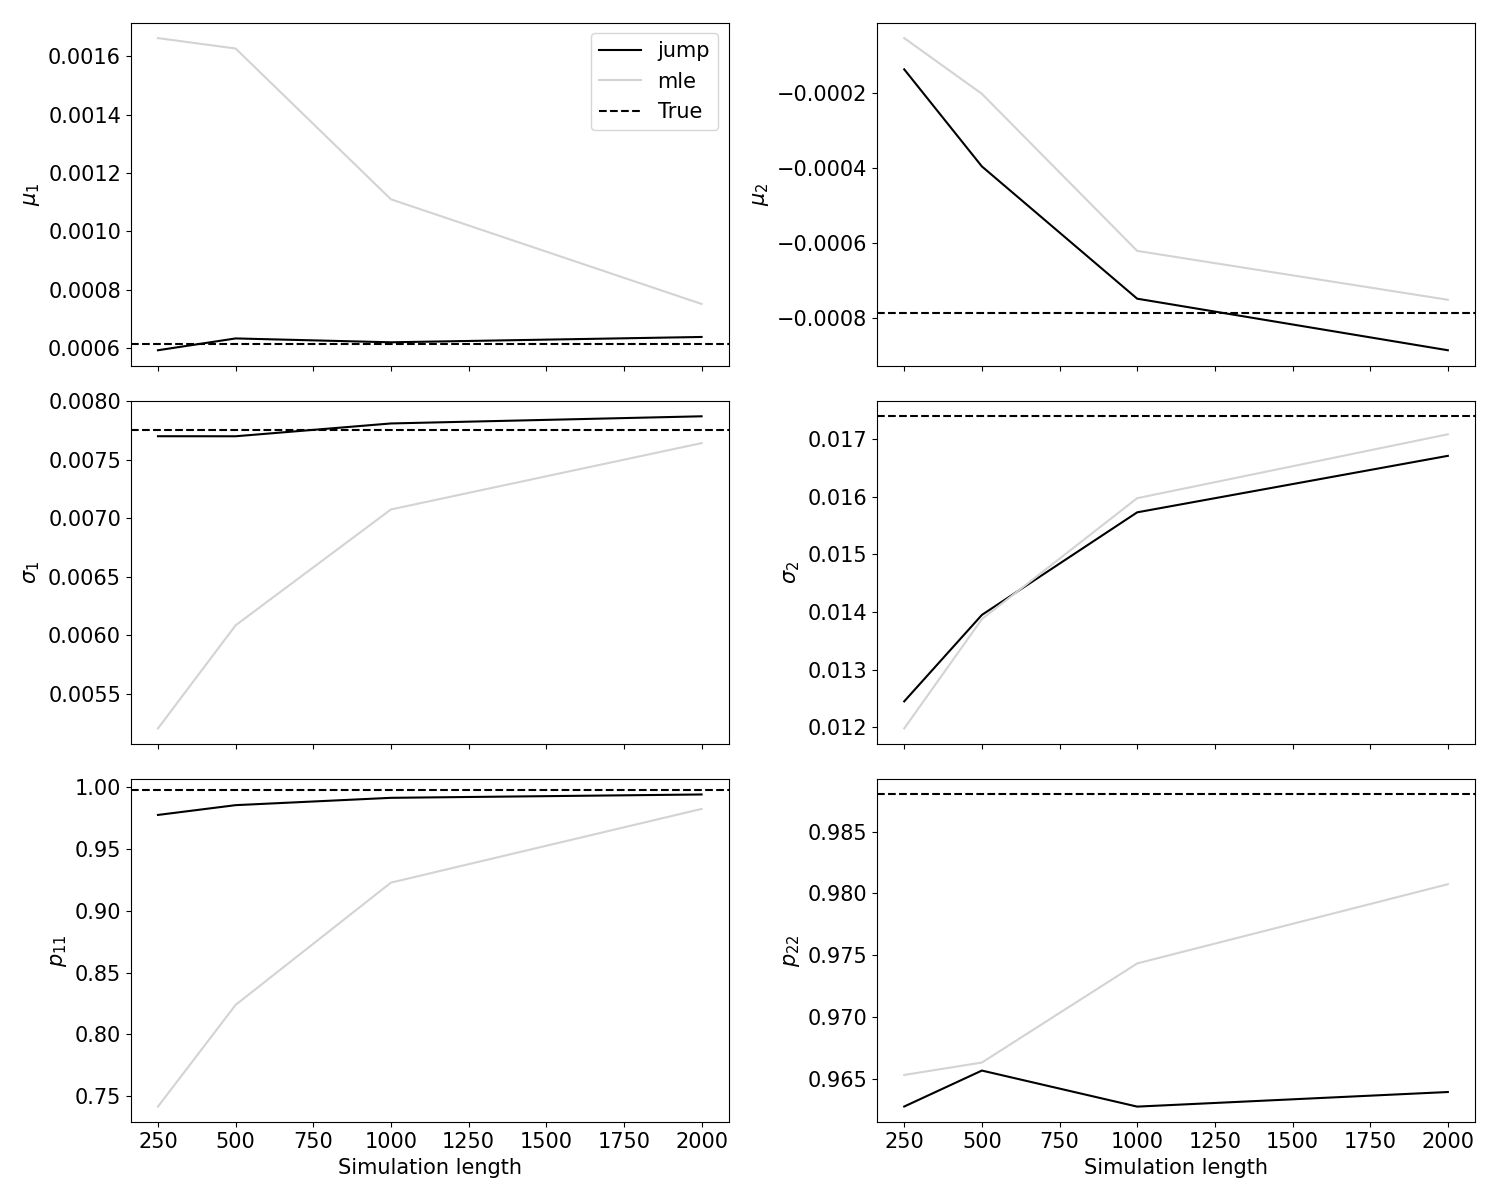
\includegraphics[width=1\textwidth]{analysis/model_convergence/images/simulation_normal.png}
    \caption{Hyper-tuning.}
    %\label{fig:jump_penalties}
\end{figure}

\begin{table}[H]
\centering
\caption{Estimated mean model parameters based on 1000 different simulations from conditional gaussian distributions}
\begin{tabular}{llrrrrrr}
\toprule
     &      &  $\mu_1$ &  $\mu_2$ &  $\sigma_1$ &  $\sigma_2$ &  $q_{11}$ &  $q_{22}$ \\
sample_size & model &          &          &             &             &           &           \\
\midrule
250  & true &   0.0006 &  -0.0008 &      0.0078 &      0.0174 &    0.9979 &    0.9880 \\
     & mle &   0.0017 &  -0.0000 &      0.0052 &      0.0121 &    0.7410 &    0.9658 \\
     & jump &   0.0006 &  -0.0001 &      0.0079 &      0.0113 &    0.9770 &    0.8903 \\
500  & true &   0.0006 &  -0.0008 &      0.0078 &      0.0174 &    0.9979 &    0.9880 \\
     & mle &   0.0015 &  -0.0002 &      0.0060 &      0.0139 &    0.8152 &    0.9719 \\
     & jump &   0.0006 &  -0.0003 &      0.0079 &      0.0130 &    0.9834 &    0.8898 \\
1000 & true &   0.0006 &  -0.0008 &      0.0078 &      0.0174 &    0.9979 &    0.9880 \\
     & mle &   0.0011 &  -0.0006 &      0.0071 &      0.0160 &    0.9208 &    0.9763 \\
     & jump &   0.0006 &  -0.0006 &      0.0080 &      0.0152 &    0.9866 &    0.9420 \\
2000 & true &   0.0006 &  -0.0008 &      0.0078 &      0.0174 &    0.9979 &    0.9880 \\
     & mle &   0.0008 &  -0.0007 &      0.0076 &      0.0171 &    0.9823 &    0.9817 \\
     & jump &   0.0006 &  -0.0007 &      0.0080 &      0.0164 &    0.9951 &    0.9679 \\
\bottomrule
\end{tabular}

\end{table}

 
\subsection{Simulation study with misspecified distributions}

\begin{figure}[H] 
    \centering
    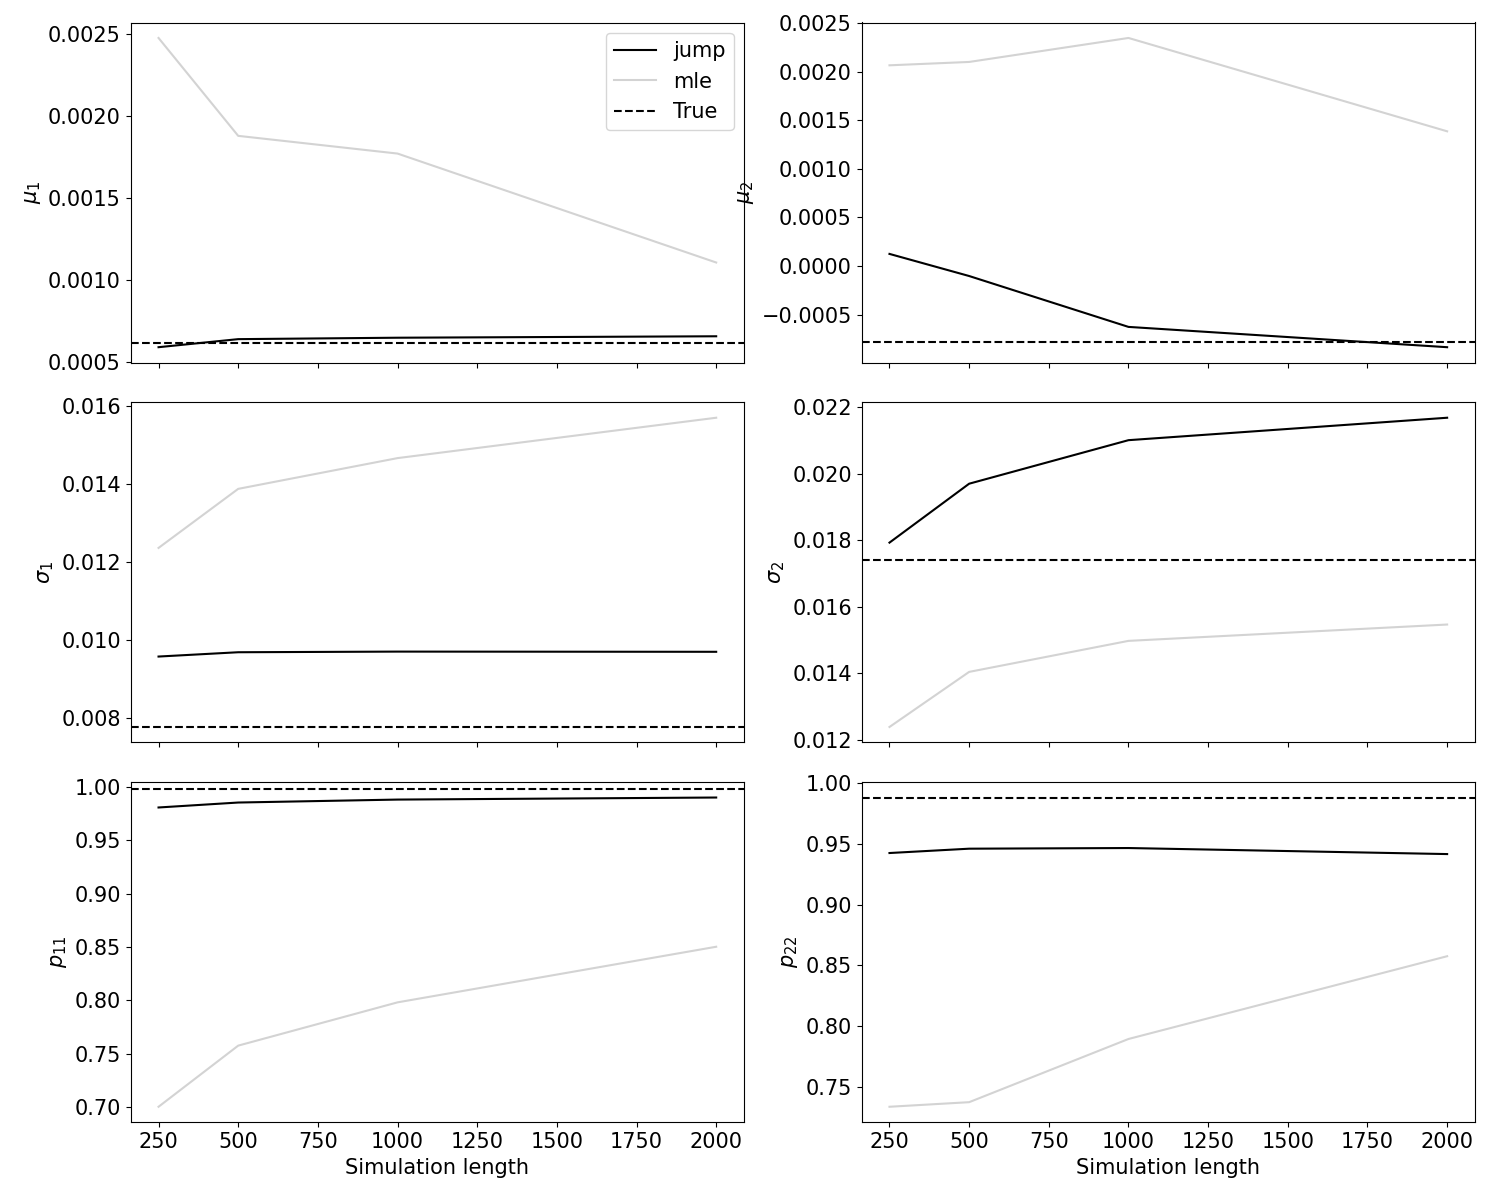
\includegraphics[width=1\textwidth]{analysis/model_convergence/images/simulation_t.png}
    \caption{Estimated mean model parameters based on 1000 different simulations from conditional t-distributions with five degrees of freedom}
    %\label{fig:jump_penalties}
\end{figure}

\begin{table}[H]
\centering
\caption{Estimated mean model parameters based on 1000 different simulations from conditional t-distributions}
\begin{tabular}{llrrrrrr}
\toprule
     &      &   $\mu_1$ &   $\mu_2$ &  $\sigma_1$ &  $\sigma_2$ &    $q_11$ &    $q_22$ \\
sample_size & model &           &           &             &             &           &           \\
\midrule
250  & true &  0.000615 & -0.000785 &    0.007759 &    0.017397 &  0.997900 &  0.988000 \\
     & mle &  0.002475 &  0.002068 &    0.012354 &    0.012383 &  0.700296 &  0.733797 \\
     & jump &  0.000591 &  0.000125 &    0.009567 &    0.017927 &  0.980719 &  0.942377 \\
500  & true &  0.000615 & -0.000785 &    0.007759 &    0.017397 &  0.997900 &  0.988000 \\
     & mle &  0.001878 &  0.002102 &    0.013870 &    0.014039 &  0.757573 &  0.737563 \\
     & jump &  0.000640 & -0.000103 &    0.009677 &    0.019699 &  0.985360 &  0.945942 \\
1000 & true &  0.000615 & -0.000785 &    0.007759 &    0.017397 &  0.997900 &  0.988000 \\
     & mle &  0.001769 &  0.002351 &    0.014671 &    0.014961 &  0.797976 &  0.789653 \\
     & jump &  0.000648 & -0.000627 &    0.009694 &    0.021009 &  0.988130 &  0.946477 \\
2000 & true &  0.000615 & -0.000785 &    0.007759 &    0.017397 &  0.997900 &  0.988000 \\
     & mle &  0.001107 &  0.001388 &    0.015695 &    0.015464 &  0.850219 &  0.857551 \\
     & jump &  0.000657 & -0.000836 &    0.009689 &    0.021683 &  0.990051 &  0.941516 \\
\bottomrule
\end{tabular}

\end{table}